%%
%% kit-prog-tutorial
%%
%% Slides for my Java programming tutorial at KIT using LaTeX beamer.
%%
%% Copyright (c) 2015-2016 YouniS Bensalah <younis.bensalah@gmail.com>
%%
%% This work is released to the public domain.
%% For the full copyright and license information, please view the LICENSE file.
%%

\documentclass[18pt]{beamer}

\usepackage{templates/beamerthemekit}

\usepackage[utf8]{inputenc}
\usepackage{hyperref}
\usepackage{listings}

%\titleimage{bauplan}
%\titleimage{greendrop}
%\titleimage{bluedrop}
%\titleimage{pinkdrop}
%\titleimage{fall}
%\titleimage{forestleaves}
%\titleimage{coloredtrees}
\titleimage{road}
%\titleimage{sortedleaves}
%\titleimage{topviewtrees}

\newcommand{\tagline}{Hello, object-oriented world!}

\title[Programmieren\hspace{2.5pt}--\hspace{2.5pt}\tagline]{\tagline}
\subtitle{Programmieren~\textbar~Tutorium 32}

\author{YouniS Bensalah}
\date{31. Oktober 2016}

\institute{Chair for Software Design and Quality}

\usepackage[citestyle=authoryear,bibstyle=numeric,hyperref,backend=biber]{biblatex}
\addbibresource{templates/example.bib}
\bibhang1em

\begin{document}

% remove annoying figure prefix in caption
\setbeamertemplate{caption}{\raggedright\insertcaption\par}

\selectlanguage{english}

\begin{frame}
    \titlepage
\end{frame}

% \begin{frame}{Heute}
%     \tableofcontents
% \end{frame}

\section{Organisatorisches}

\subsection{Hi}

\begin{frame}{Hi}
    \begin{itemize}
        \item \textbf{Younis Bensalah}
        \item Bachelor Informatik
        \item 5. Semester
        \item \url{<younis.bensalah@gmail.com>}
    \end{itemize}
\end{frame}

\subsection{Übungsbetrieb}

\begin{frame}{Folien, Übungsblätter etc.}
    \begin{itemize}
        \item \textbf{Vorlesungsunterlagen und Übungsblätter}
        \begin{itemize}
            \item \url{https://sdqweb.ipd.kit.edu/wiki/Vorlesung_Programmieren_WS16/17}
        \end{itemize}

        \vspace{.1in}

        \item \textbf{Tutoriumsfolien}
        \begin{itemize}
            \item Im ILIAS unter \textit{Tutorien}
            \item \url{https://ilias.studium.kit.edu/ilias.php?ref_id=614188&cmd=view&cmdClass=ilrepositorygui&cmdNode=75&baseClass=ilrepositorygui}
        \end{itemize}
    \end{itemize}
\end{frame}

\begin{frame}{Modul Programmieren auf Twitter\dots}
    \begin{figure}
        
\includegraphics[scale=.4]{img/modulprogtwitter.png}
    \end{figure}
\end{frame}

\begin{frame}{Disclaimer}
    \begin{itemize}
        \item \textbf{Frist: \alert{06.11.2016}}
        \item Unterschreiben und in den Programmieren-Briefkasten werfen
        \item Info-Bau (50.34) 1. UG
    \end{itemize}
\end{frame}

\begin{frame}{Übungsblätter und Präsenzübung}
    \begin{block}{Übungsblätter}
        \begin{itemize}
            \item \textbf{5} Übungsblätter
            \item \textbf{2} Wochen Bearbeitungszeit
            \item Abgabe (exklusiv) über Praktomat
            \item Ungefähr \textbf{100} Punkte insgesamt (20 je Blatt)
            \item $>$\textbf{50}$\%$ hinreichend
        \end{itemize}
    \end{block}

    \pause

    \begin{block}{Präsenzübung}
        \begin{itemize}
            \item Schriftliche Prüfung ($\sim$20 Minuten)
            \item $>$\textbf{75}$\%$ hinreichend
            \item Findet am \textbf{25.01.2017} statt
        \end{itemize}
    \end{block}


\end{frame}

\begin{frame}{Übungsschein}
    \begin{itemize}
        \item \textbf{Übungsschein = \alert{5}} Übungsblätter + \textbf{\alert{1}} Präsenzübung
        \pause
        \item \alert{Vorraussetzung für Abschlussaufgaben}
        \pause
        \item Übungsblätter oder Präsenzübung \textit{nicht} bestanden
        \begin{itemize}
            \item kein Schein, beides wiederholen
        \end{itemize}
        \pause
        \item Ausnahme: Rücktritt von Präsenzübung aus triftigem Grund
        \begin{itemize}
            \item kein Schein, nur Präsenzübung wiederholen
        \end{itemize}
    \end{itemize}

\end{frame}

\begin{frame}{Abschreiben, Betrug etc.}
    \begin{alertblock}{Abschreiben, Betrug etc.}
        \begin{itemize}
            \item Ihr lernt nichts dabei
            \pause
            \item Ihr werdet erwischt
            \pause
            \item Sofort 5.0
            \pause
            \item 2. Betrugsversuch $\rightarrow$ Exmatrikulation
        \end{itemize}
    \end{alertblock}
\end{frame}


\begin{frame}{Bewertungskriterien}
    \begin{enumerate}
        \item Funktionalität
        \item Modellierung
        \item Methodik
        \item Dokumentation
        \item Lesbarkeit
    \end{enumerate}
\end{frame}


\begin{frame}{Orientierungsprüfung}
    \begin{itemize}
        \item \textbf{Modul Programmieren} ist \textbf{Orientierungsprüfung}!
        \begin{itemize}
            \item Bis zum 2. Semester antreten
            \item Bis zum 3. Semester bestehen
        \end{itemize}

    \end{itemize}
\end{frame}


\subsection{Praktomat}

\begin{frame}{Praktomat}
    \begin{block}{Praktomat}
        \begin{itemize}
            \item Hier gebt ihr die Übungsaufgaben ab
            \item Zugang mit KIT-Account (uxxxx)
            \item \alert{Umgehend anmelden!}
            \item \url{https://praktomat.cs.kit.edu/2016_WS}
        \end{itemize}
    \end{block}

\end{frame}


\subsection{VPN}

\begin{frame}{VPN}
    \begin{itemize}
        \item \textbf{\alert{Praktomat nur aus dem KIT-Netz erreichbar}}
        \item Möglichkeit, von außerhalb (z.B. von zu Hause) eine Verbindung mit dem KIT-Netz herzustellen
        \item Zugang mit KIT-Account (uxxxx)
        \item Anleitung hier: \url{https://www.scc.kit.edu/dienste/vpn.php}
    \end{itemize}
\end{frame}


\subsection{ILIAS}

\begin{frame}{ILIAS}
    \begin{block}{ILIAS}
        \begin{itemize}
            \item \textbf{Forum zu Vorlesung und Übungsaufgaben}
            \item Login via KIT-Account (uxxxx)
            \item Kurs \textit{Programmieren} beitreten
            \item \url{https://ilias.studium.kit.edu}
        \end{itemize}
    \end{block}
\end{frame}


\section{Java}

\subsection{JDK}

\begin{frame}{Java Development Kit}
    \begin{block}{Installation}
        \begin{itemize}
            \item Version \textbf{8}
            \item Oracle JDK oder OpenJDK
            \pause
            \item Windows
            \begin{itemize}
                \item JDK hier downloaden:\\
                \url{http://www.oracle.com/technetwork/java/javase/downloads/jdk8-downloads-2133151.html}
                \item \url{PATH} Variable setzen
            \end{itemize}
            \item Mac
            \begin{itemize}
                \item JDK bereits vorinstalliert
            \end{itemize}
            \item Linux
            \begin{itemize}
                \item Via package manager
                \item \url{openjdk-8-jdk} oder \url{jdk8-openjdk} oder\dots
            \end{itemize}
        \end{itemize}
    \end{block}
\end{frame}

\subsection{Code-Editor}

\begin{frame}{Code-Editor}
    \begin{itemize}
        \item Zum Verfassen von Java-Sourcecode
        \item Im Prinzip freie Wahl
        \item \textit{Syntax Highlighting} ist eine gute Idee
        \item Besser noch keine IDEs verwenden
    \end{itemize}
\end{frame}


\begin{frame}{Atom (\url{atom.io})}

    \begin{itemize}
        \item Cross platform
        \item Open source
        \item Plugins\dots
    \end{itemize}

    \begin{figure}
        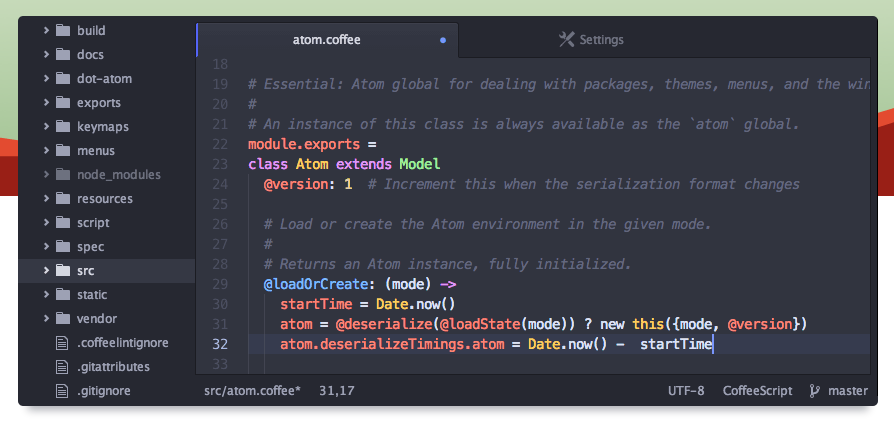
\includegraphics[scale=.38]{img/atom.png}
        \caption{atom.io}
    \end{figure}
\end{frame}


\subsection{Vom Quelltext zum laufenden Programm}

\begin{frame}{Vom Quelltext zum laufenden Programm}
    \begin{figure}
        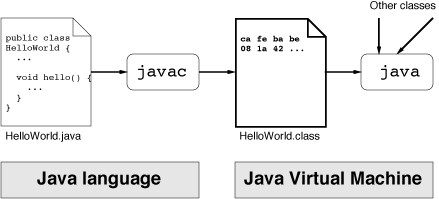
\includegraphics[scale=0.7]{img/jvm.png}
    \end{figure}
\end{frame}

\begin{frame}{Hello World in Java}
    \begin{enumerate}
        \item Schreibe folgenden Java-Sourcecode in Editor ab
        \item Quelltext-Datei als \texttt{Hello.java} abspeichern
        \item Kompilieren
            \begin{itemize}
                \item \texttt{javac Hello.java}
            \end{itemize}
        \item Ausführen
        \begin{itemize}
            \item \texttt{java Hello}
        \end{itemize}
    \end{enumerate}
\end{frame}

\begin{frame}[fragile]{Hello World in Java}
    \begin{lstlisting}[language=Java]
public class Hello {
    public static void main(String[] args) {
        System.out.println("Hello, world!");
    }
}
    \end{lstlisting}
\end{frame}

\section{Objektorientierte Programmierung}

\subsection{Objektorientierung}

\begin{frame}{Objektorientierung}
    \begin{figure}
        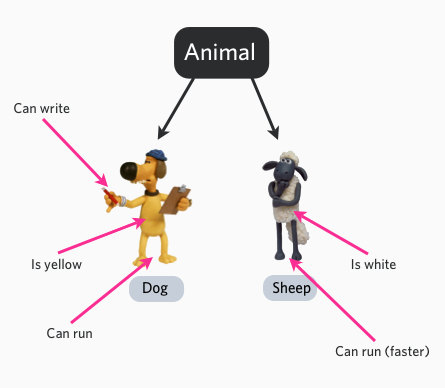
\includegraphics[scale=0.4]{img/animalclass.png}
    \end{figure}
\end{frame}

\begin{frame}{Objektorientierung}
    Worum geht es bei \textbf{Objektorientierung}?
    \pause
    \begin{itemize}
        \item Abstraktion der realen Welt
        \pause
        \item Beschreibung komplexer Systeme durch das Zusammenspiel kooperierender Objekte
        \pause
        \item Modellierung realer Objekte
        \pause
        \item Modellieren $\ne$ Programmieren
    \end{itemize}
    \vspace{.2in}
    \textit{Hier ist noch nicht die Rede von Programmieren.}
\end{frame}

\begin{frame}{Objektorientierung}
    Was versteht man unter einem \textbf{Objekt}?
    \pause
    \begin{itemize}
        \item Alles kann ein Objekt sein
        \pause
        \item Die Frage ist vielmehr: \textit{Ist es sinnvoll?}
        \pause
        \item Ein Objekt \textit{besitzt} \textbf{Attribute} und \textit{beherrscht} \textbf{Methoden}
        \pause
        \item \textit{Welche} hängt von der Modellierung ab
    \end{itemize}
\end{frame}

\begin{frame}{Methoden und Attribute}
    \begin{block}{Methoden}
        Methoden sind die \textbf{Aktionen}, welche ein Objekt ausführen kann
    \end{block}
    \pause
    \begin{block}{Attribute}
        Attribute sind die \textbf{Eigenschaften}, die den Zustand eines Objekts definieren
    \end{block}
\end{frame}

\begin{frame}{Methoden und Attribute}
    \begin{exampleblock}{Methoden}
        \begin{itemize}
            \item Eine \textbf{Kaffeemaschine} kann \textbf{Kaffee kochen}
            \item Ein \textbf{Auto} kann \textbf{fahren}
            \item Ein \textbf{GPS} kann eine \textbf{Route berechnen}
        \end{itemize}
    \end{exampleblock}
    \pause
    \begin{exampleblock}{Attribute}
        \begin{itemize}
            \item Eine \textbf{Kaffeemaschine} hat einen \textbf{Wasserstand}
            \item Ein \textbf{Auto} hat einen aktuellen \textbf{Tachowert}
            \item Ein \textbf{GPS} hat eine \textbf{aktuelle Position}
        \end{itemize}
    \end{exampleblock}
\end{frame}

\begin{frame}{Beispiel: Bibliothek}
    \begin{figure}
        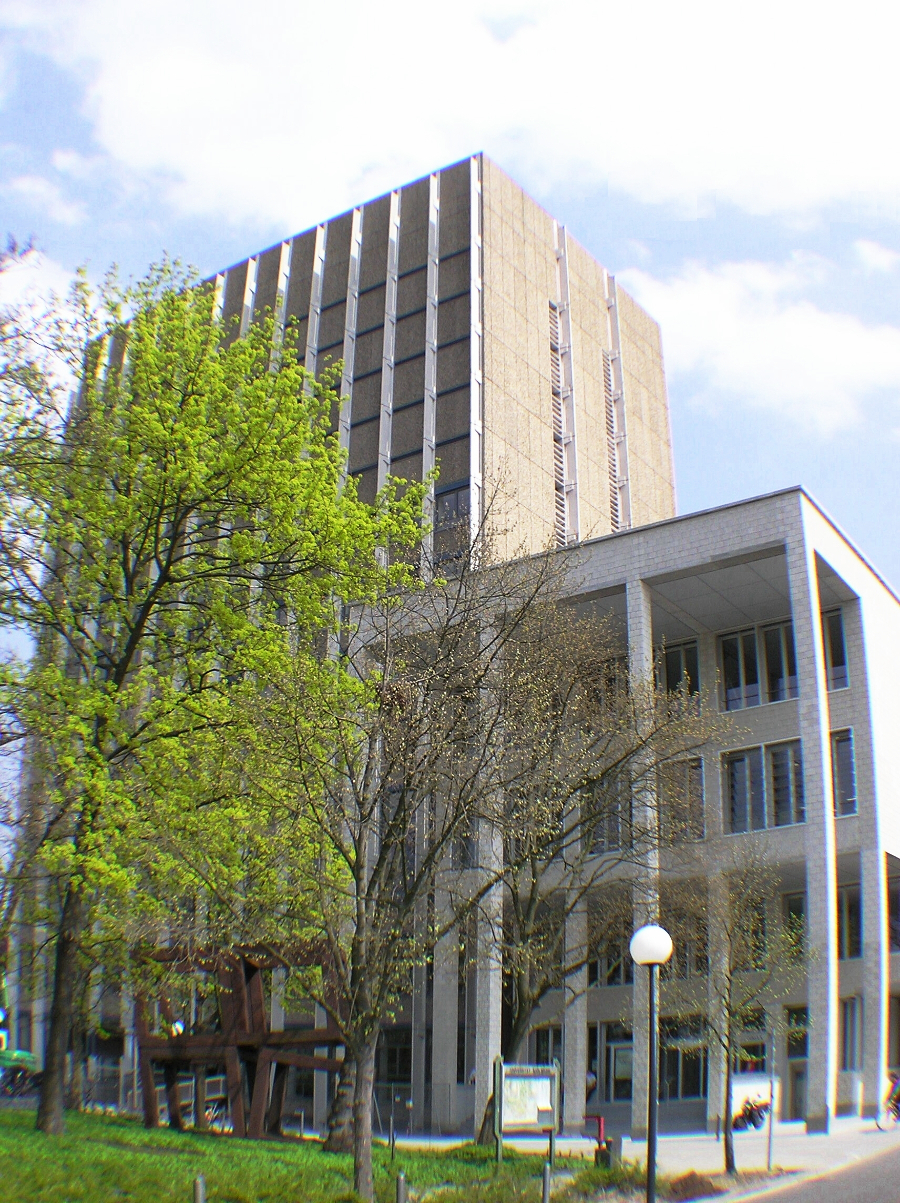
\includegraphics[scale=0.15]{img/kit_bib_sued.jpg}
    \end{figure}
\end{frame}

\begin{frame}{Bibliothek - Modellierungsversuch}
    Ziel: \textbf{Modellierung einer Bibliothek}\\
    \vspace{.1in}
    Dabei kommen einige Fragen auf\dots
    \pause
    \begin{itemize}
        \item Eine Bibliothek ist ein komplexes System
        \begin{itemize}
            \item Welche Aspekte möchten wir in unserem Modell beibehalten?
            \item Welche Details möchten wir dabei ausblenden?
            \item Welche Informationen interessieren uns?
            \item Wie weit dürfen wir das Modell vereinfachen?
        \end{itemize}
        \pause
        \item Eine Bibliothek besteht aus kleineren Teilsystemen
        \begin{itemize}
            \item Wie tief muss ich diese Hierarchie beibehalten?
            \item Wie hängen diese Teilsysteme miteinander zusammen?
        \end{itemize}
    \end{itemize}
\end{frame}

\begin{frame}{Bibliothek - Modellierungsversuch}
    Problem: Wir können diese Fragen noch nicht beantworten!\\
    Vorher: \textbf{Wozu soll das Modell verwendet werden?}
    \pause
    \begin{itemize}
        \item Erstellen eines Wegweisers für die Bibliothek
        \item Verwaltung von Besuchern, Studenten, Mitarbeitern\dots
        \item Eintrag im Telefonbuch
        \item Versand von Büchern
        \item Erstellen eines Stadtplans, Campusplans\dots
        \item Ausleihen und Einordnen von Büchern
        \item Einrichten eines internen Rechnernetzes
        \item Installation eines Wasserspenders
    \end{itemize}
\end{frame}

\begin{frame}{Bibliothek - Modellierungsversuch}
    \begin{itemize}
        \item Erstellen eines Wegweisers für die Bib
        \begin{itemize}
            \item Grundriss des Gebäudes: \textbf{relevant}
            \item Wo stehen welche Themengebiete: \textbf{relevant}
            \item Welche Bücher sind zurzeit verfügbar: \textbf{weniger relevant}
            \item Höhe der Decke: \textbf{noch weniger relevant}
        \end{itemize}
        \pause
        \item Als Eintrag im Telefonbuch
        \begin{itemize}
            \item Telefonnummer der Bib: \textbf{relevant}
            \item Anschrift: \textbf{relevant}
            \item Grundriss des Gebäudes: \textbf{nicht relevant}
        \end{itemize}
        \pause
        \item Ausleihen von Büchern
        \begin{itemize}
            \item Welche Bücher sind zurzeit verfügbar: \textbf{relevant}
            \item Grundriss des Gebäudes: \textbf{kann relevant sein}
            \item Raumtemperatur: \textbf{nicht relevant}
        \end{itemize}
    \end{itemize}
    You get the idea\dots
\end{frame}

\begin{frame}{Bibliothek - Modellierungsversuch}
    \textbf{Wie könnte eine geeignete Modellierung (Objekte, Methoden, Attribute) der \textbf{Bibliothek} für folgendes Szenario aussehen?}
    \vspace{.1in}
    \begin{itemize}
        \item Bibliothek stellt Studenten eine Reihe von Büchern zur Verfügung
        \item Studenten können sich in der Bibliothek anmelden können
        \item Studenten sollen Bücher ausleihen können
        \item Studenten müssen anfallende Gebühren zurückzahlen
    \end{itemize}
\end{frame}

\begin{frame}{Bibliothek - Modellierungsversuch}
    \textbf{Ein paar mögliche Stichpunkte:}
    \begin{itemize}
        \item \textbf{Bibliothek}
        \begin{itemize}
            \item hat Liste aller verfügbaren Bücher
            \item hat Liste aller angemeldeten Studenten
            \item führt Buch über ausgeliehene Bücher (Student, Buch, Datum\dots)
            \item führt Buch über Gebühren
            \item erlaubt das Ausleihen von Büchern an Studentens
            \item erlaubt das Bezahlen von Gebühren
        \end{itemize}
        \pause
        \item \textbf{Student}
        \begin{itemize}
            \item Name, Matrikelnummer, E-Mail
            \item kann Bücher ausleihen
            \item kann Gebühren zahlen
        \end{itemize}
        \pause
        \item \textbf{Buch}
        \begin{itemize}
            \item Titel, ISBN, Regal, Anzahl verfügbarer Exemplare
            \item kann ausgeliehen werden
            \item kann zurückgebracht werden
        \end{itemize}
    \end{itemize}
\end{frame}

\subsection{Objektorientierte Programmierung in Java}

\begin{frame}{Objektorientierte Programmierung}
    Wir übertragen jetzt dieses Konzept auf die Programmierung in Java
\end{frame}

\begin{frame}{Klassen}
    \begin{block}{Klasse}
        Eine \textbf{Klasse} beschreibt das \textbf{abstrakte Modell} für eine Reihe von ähnlichen Objekten
    \end{block}

    \begin{block}{Objekt}
        Ein \textbf{Objekt} ist eine \textbf{konkrete Ausprägung} einer Klasse
    \end{block}
\end{frame}

\begin{frame}[fragile]{Klassen und Objekte}
    Man definiert eine Klasse in Java mit \texttt{class}
    \begin{exampleblock}{}
        \begin{lstlisting}[language=Java]
class Student {

    // attributes...

    // methods...

}
        \end{lstlisting}
    \end{exampleblock}
\end{frame}

\begin{frame}[fragile]{Klassen und Objekte}
    \begin{itemize}
        \item \textbf{Instanziierung} = das Erzeugen eines Objekts von einer Klasse
        \item Man \textit{instanziiert} eine Klasse und erhält ein \textbf{Objekt}
    \end{itemize}

    \begin{exampleblock}{}
        \begin{lstlisting}[language=Java]
Student ersti = new Student();
        \end{lstlisting}
    \end{exampleblock}
\end{frame}

\begin{frame}{Haus-Analogie}
    \begin{itemize}
        \item Die \textbf{Klasse} ist der \textbf{Bauplan}
        \item Die \textbf{Objekte} sind die fertigen \textbf{Häuser}
    \end{itemize}
\end{frame}

\begin{frame}{Klasse vs. Objekt}
    \begin{figure}
        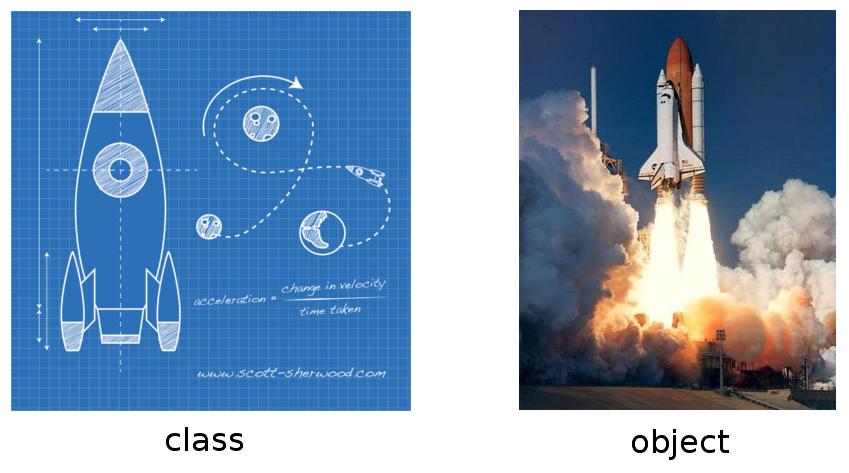
\includegraphics[scale=0.3]{img/classvsobject.png}
    \end{figure}
\end{frame}

\subsection{Attribute}

\begin{frame}{Attribute}
    \begin{itemize}
        \item Attribute definieren den Zustand eines Objekts
        \item Verschiedene Objekte vom gleichen Typ haben verschiedene Zustände
        \item \textit{Es gibt verschiedene Ampeln, aber nicht alle sind gleichzeitig Grün}
    \end{itemize}
\end{frame}

\begin{frame}[fragile]{Attribute}
    \begin{exampleblock}{}
        \begin{lstlisting}[language=Java]
class Student {

    private int semester;

}
        \end{lstlisting}
    \end{exampleblock}
\end{frame}

\subsection{Methoden}

\begin{frame}{Methoden}
    \begin{itemize}
        \item Methoden beschreiben das Verhalten von Objekten
        \item Alle Objekte vom gleichen Typ können die gleichen Funktionen ausführen
        \item \textit{Alle Ampeln können von Rot auf Grün schalten}
    \end{itemize}
\end{frame}

\begin{frame}[fragile]{Methoden}
    \begin{exampleblock}{}
        \begin{lstlisting}[language=Java]
class Student {

    public void study() {
        // ...
    }

}
        \end{lstlisting}
    \end{exampleblock}
\end{frame}

\begin{frame}[fragile]{Methodenaufruf}
    \begin{exampleblock}{}
        \begin{lstlisting}[language=Java]
Student ersti = new Student();

ersti.study();
        \end{lstlisting}
    \end{exampleblock}
\end{frame}

\begin{frame}{Rückgabewert}
    Eine Methode darf einen Wert zurückgeben
    \begin{itemize}
        \item Schlüsselwort \texttt{return}
        \item Der Rückgabewert wird an den Aufrufer weitergereicht
        \item \texttt{void} bedeutet ``kein Rückgabetyp''
    \end{itemize}

\end{frame}

\begin{frame}[fragile]{Rückgabewert}
    \begin{exampleblock}{Beispiel 1}
        \begin{lstlisting}[language=Java]
double temperature = cpu.getTemperature();
        \end{lstlisting}
    \end{exampleblock}
\end{frame}

\begin{frame}[fragile]{Rückgabewert}
    \begin{exampleblock}{Beispiel 2}
        \begin{lstlisting}[language=Java]
public int sum(int a, int b) {
    return a + b;
}
        \end{lstlisting}
    \end{exampleblock}
\end{frame}

\begin{frame}[fragile]{Main}
    Die \texttt{main} Methode markiert den Startpunkt des Programms
    \begin{lstlisting}[language=Java]
class Main {
    public static void main(String[] args) {
        // ...
    }
}
    \end{lstlisting}
\end{frame}

\appendix

\beginbackup

\begin{frame}{Fragen?}
    \begin{figure}
        
\includegraphics[scale=.3]{img/fragen.jpg}
    \end{figure}
\end{frame}

\begin{frame}{Bis nächste Woche!}
    \begin{figure}
        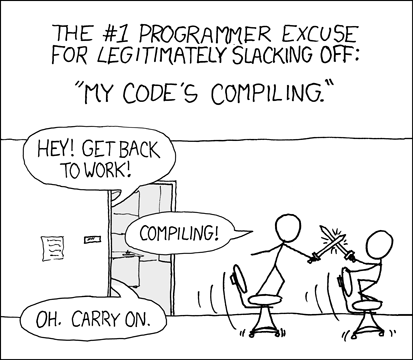
\includegraphics[scale=.4]{img/compiling.png}
        \caption{\footnotesize{xkcd.com}}
    \end{figure}
\end{frame}

\backupend

\end{document}
